\section{RL for Device Placement}

% ---------------------------------------------------------------- Divider
\begin{frame}{}
    \LARGE RL for \textbf{Device Placement}
\end{frame}

% ---------------------------------------------------------------- Slide 33
\begin{frame}{What is device placement and why is it important?}
\begin{center}
{\large Trend towards many-device training, bigger models, larger batch sizes}
\end{center}
\vfill
\begin{columns}[c]
\begin{column}{0.34\textwidth}
\centering
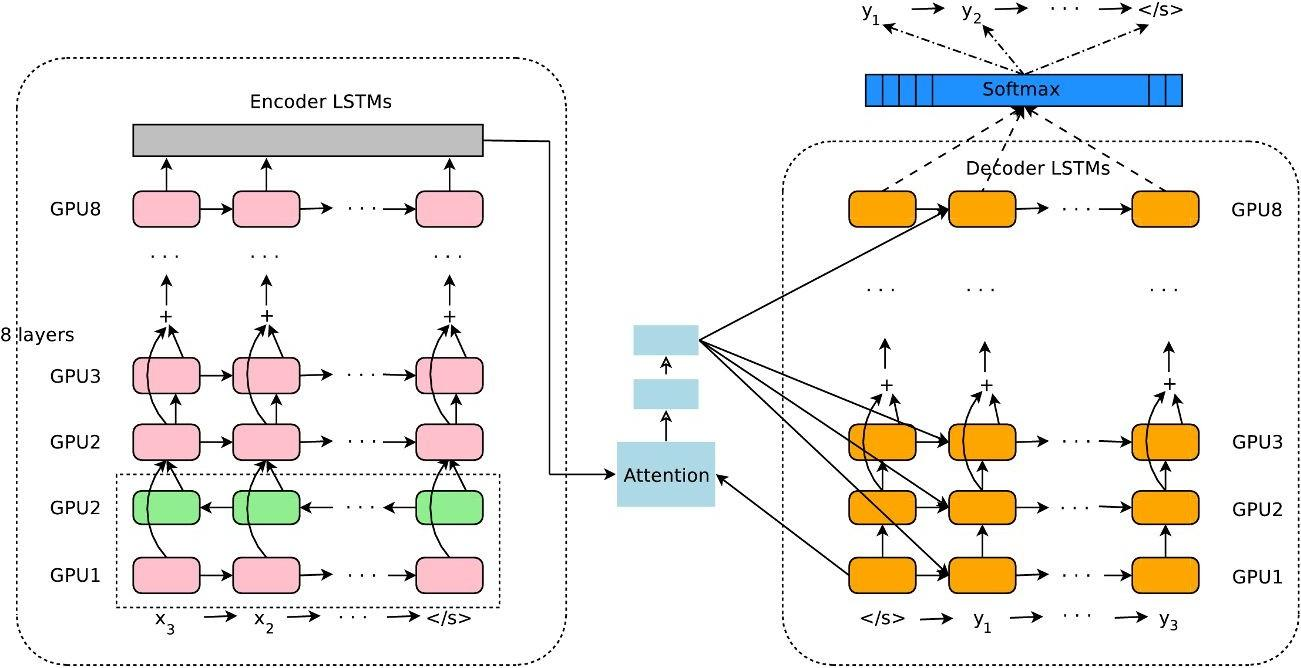
\includegraphics[width=\linewidth,height=0.42\textheight,keepaspectratio]{images/rl-real-world/figures/device-model-1.jpg}\\[0.4em]
{\scriptsize Google neural machine translation '16\\ 300 million parameters,
trained on 128 GPUs}
\end{column}
\begin{column}{0.34\textwidth}
\centering
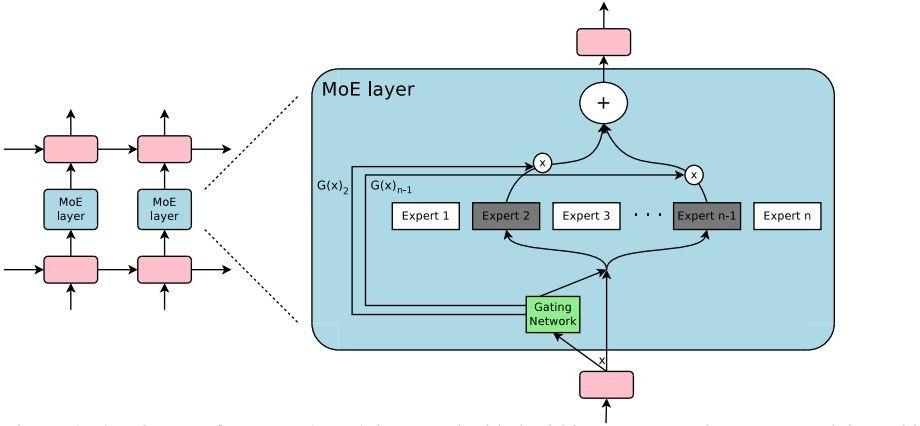
\includegraphics[width=\linewidth,height=0.42\textheight,keepaspectratio]{images/rl-real-world/figures/device-model-2.jpg}\\[0.4em]
{\scriptsize Sparsely gated mixture of experts '17\\ 130 billion parameters,
trained on 128 GPUs}
\end{column}
\begin{column}{0.30\textwidth}
\centering
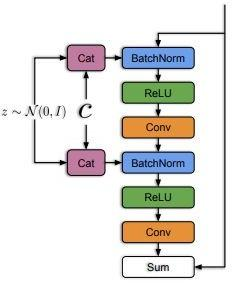
\includegraphics[width=0.7\linewidth,height=0.42\textheight,keepaspectratio]{images/rl-real-world/figures/device-model-3.jpg}\\[0.4em]
{\scriptsize BigGAN '18\\ 355 million parameters,\\ trained on 512 TPU cores}
\end{column}
\end{columns}
\end{frame}

% ---------------------------------------------------------------- Slide 34
\begin{frame}{Standard practice for device placement}
\begin{itemize}
    \item Often based on greedy heuristics
    \item Requires deep understanding of devices: nonlinear FLOPs, bandwidth, latency
          behavior
    \item Requires modeling parallelism and pipelining
    \item Does not generalize well
\end{itemize}
\end{frame}

% ---------------------------------------------------------------- Slide 35
\begin{frame}{ML for device placement}
\begin{itemize}
    \item ML is repeatedly replacing rule based heuristics
    \item RL can be applied to device placement
    \begin{itemize}
        \item Effective search across large state and action spaces to find optimal
              solutions
        \item Automated learning from underlying environment only based on reward
              function (e.g. runtime of a program)
    \end{itemize}
\end{itemize}
\end{frame}

% ---------------------------------------------------------------- Slide 36
\begin{frame}{Posing device placement as an RL problem}
\definecolor{cpupurple}{RGB}{179,179,224}
\vfill
\centering
\begin{tikzpicture}[font=\small,
    ar/.style={-{Stealth[length=3mm]}, line width=1pt, gray!60!black}]
    % section labels
    \node[gray, font=\large] at (2.4,5.0) {Input \quad RL model};
    \node[gray, font=\large] at (10.6,5.0) {Output};
    % neural model box
    \node[draw, inner sep=2pt] (nm) at (2.0,3.5)
        {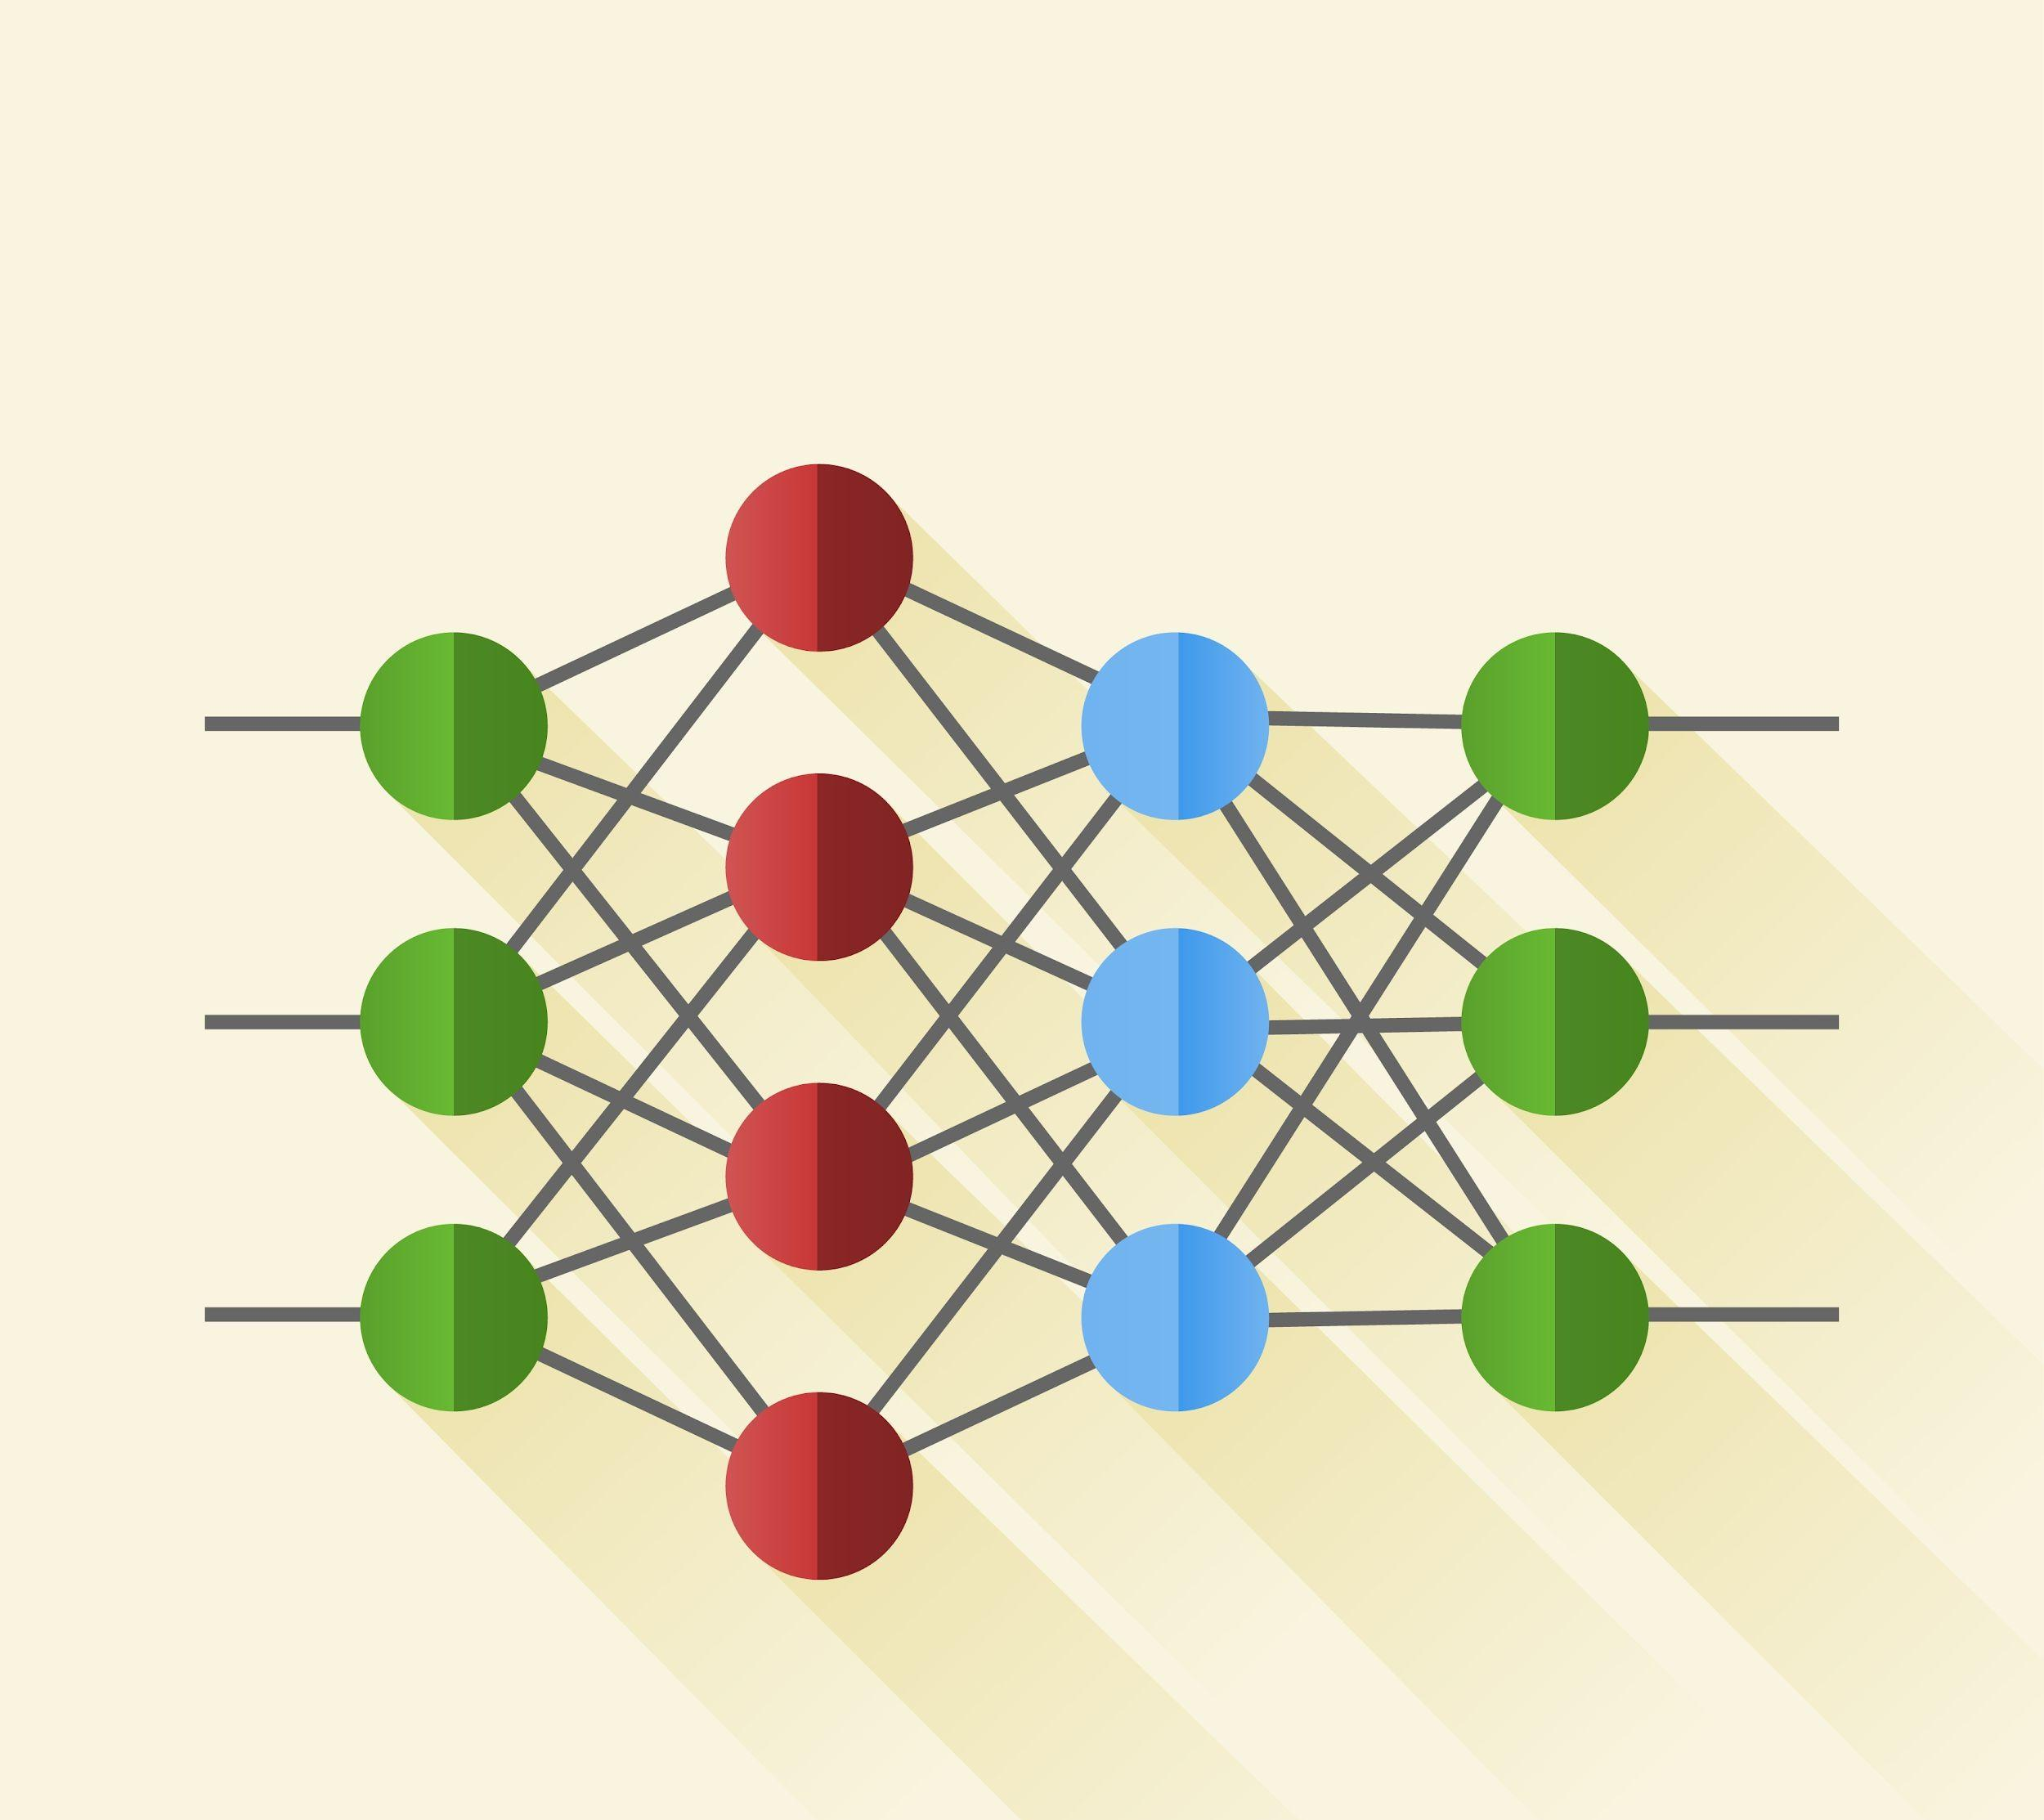
\includegraphics[width=2.6cm]{images/rl-real-world/figures/device-rl-1.jpg}};
    \node[draw, fill=white, font=\small] at (1.4,4.35) {Neural model};
    % devices box
    \node[draw, minimum width=4cm, minimum height=2.1cm] (dev) at (2.2,1.1) {};
    \node[font=\small] at (2.2,1.95) {Set of available devices};
    \foreach \i in {0,1,2}{
        \fill[cpupurple, draw=black] (0.7+0.08*\i,0.4+0.08*\i) rectangle ++(1.0,0.7);
        \fill[boxblue, draw=black]   (2.5+0.08*\i,0.4+0.08*\i) rectangle ++(1.0,0.7);
    }
    \node[font=\small] at (1.28,0.83) {CPU};
    \node[font=\small] at (3.08,0.83) {GPU};
    % policy
    \node[draw, rounded corners, fill=boxgreen, minimum width=2cm, minimum height=3.2cm] (pol) at (6.4,2.7) {Policy};
    % output box
    \node[draw, align=center, minimum width=3.2cm, minimum height=1.5cm] (out) at (10.5,2.9)
        {Assignment of ops in\\ neural model to devices};
    % arrows
    \draw[ar] (nm.east)  -- (pol.west|-nm.east);
    \draw[ar] (dev.east) -- (pol.west|-dev.east);
    \draw[ar] (pol.east) -- (out.west);
\end{tikzpicture}
\vfill
\footnote[0]{\scriptsize Mirhoseini et al. \href{https://arxiv.org/abs/1802.09756}{Hierarchical Planning for Device Placement}. ICLR 2018.}
\end{frame}

% ---------------------------------------------------------------- Slide 37
\begin{frame}{Posing device placement as an RL problem}
\definecolor{cpupurple}{RGB}{179,179,224}
\vfill
\centering
\begin{tikzpicture}[font=\small,
    ar/.style={-{Stealth[length=3mm]}, line width=1pt, gray!60!black}]
    \node[gray, font=\large] at (2.4,5.0) {Input \quad RL model};
    \node[gray, font=\large] at (10.6,5.0) {Output};
    \node[draw, inner sep=2pt] (nm) at (2.0,3.5)
        {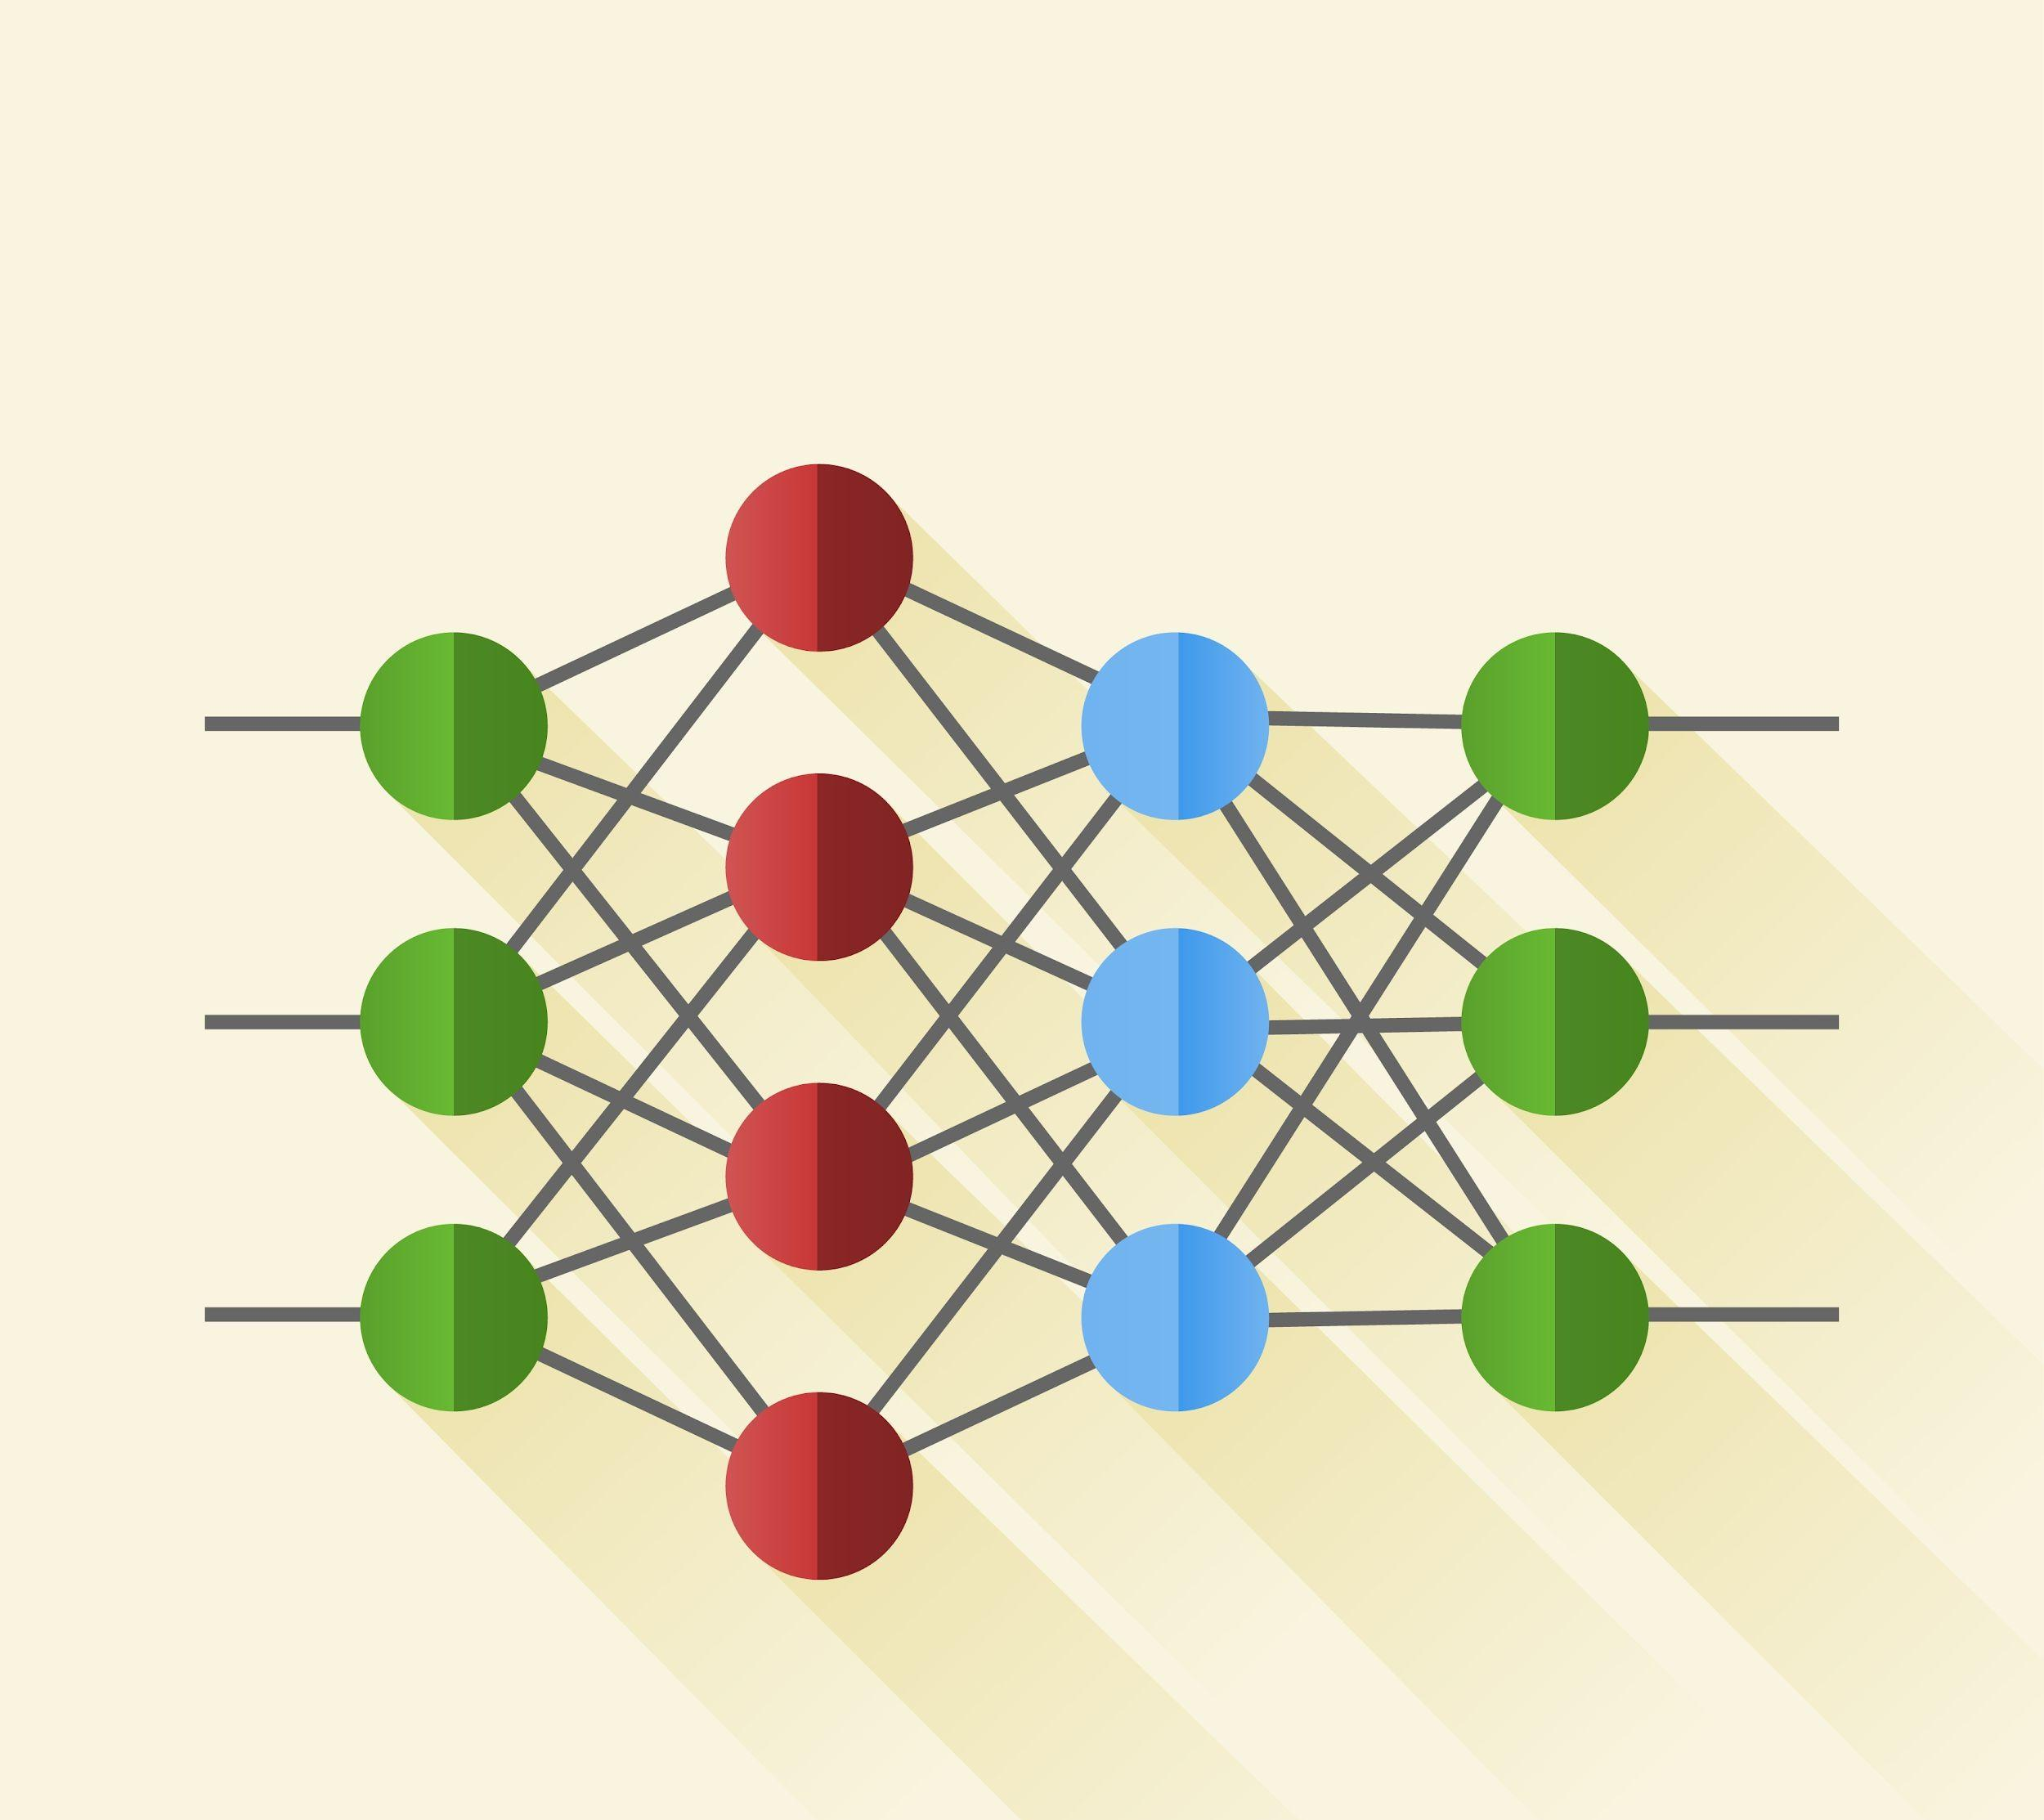
\includegraphics[width=2.6cm]{images/rl-real-world/figures/device-rl-1.jpg}};
    \node[draw, fill=white, font=\small] at (1.4,4.35) {Neural model};
    \node[draw, minimum width=4cm, minimum height=2.1cm] (dev) at (2.2,1.1) {};
    \node[font=\small] at (2.2,1.95) {Set of available devices};
    \foreach \i in {0,1,2}{
        \fill[cpupurple, draw=black] (0.7+0.08*\i,0.4+0.08*\i) rectangle ++(1.0,0.7);
        \fill[boxblue, draw=black]   (2.5+0.08*\i,0.4+0.08*\i) rectangle ++(1.0,0.7);
    }
    \node[font=\small] at (1.28,0.83) {CPU};
    \node[font=\small] at (3.08,0.83) {GPU};
    \node[draw, rounded corners, fill=boxgreen, minimum width=2cm, minimum height=3.2cm] (pol) at (6.4,2.7) {Policy};
    \node[draw, align=center, minimum width=3.2cm, minimum height=1.5cm] (out) at (10.5,2.9)
        {Assignment of ops in\\ neural model to devices};
    % evaluate-runtime feedback
    \node[draw, rounded corners, fill=boxred, align=center, minimum width=2.4cm, minimum height=1.1cm] (eval) at (8.0,-0.2) {Evaluate\\ runtime};
    \draw[ar] (nm.east)  -- (pol.west|-nm.east);
    \draw[ar] (dev.east) -- (pol.west|-dev.east);
    \draw[ar] (pol.east) -- (out.west);
    \draw[ar] (out.south) |- (eval.east);
    \draw[ar] (eval.west) -| (pol.south);
\end{tikzpicture}
\vfill
\end{frame}

% ---------------------------------------------------------------- Slide 38
\begin{frame}{An end-to-end hierarchical placement model}
\vfill
\centering
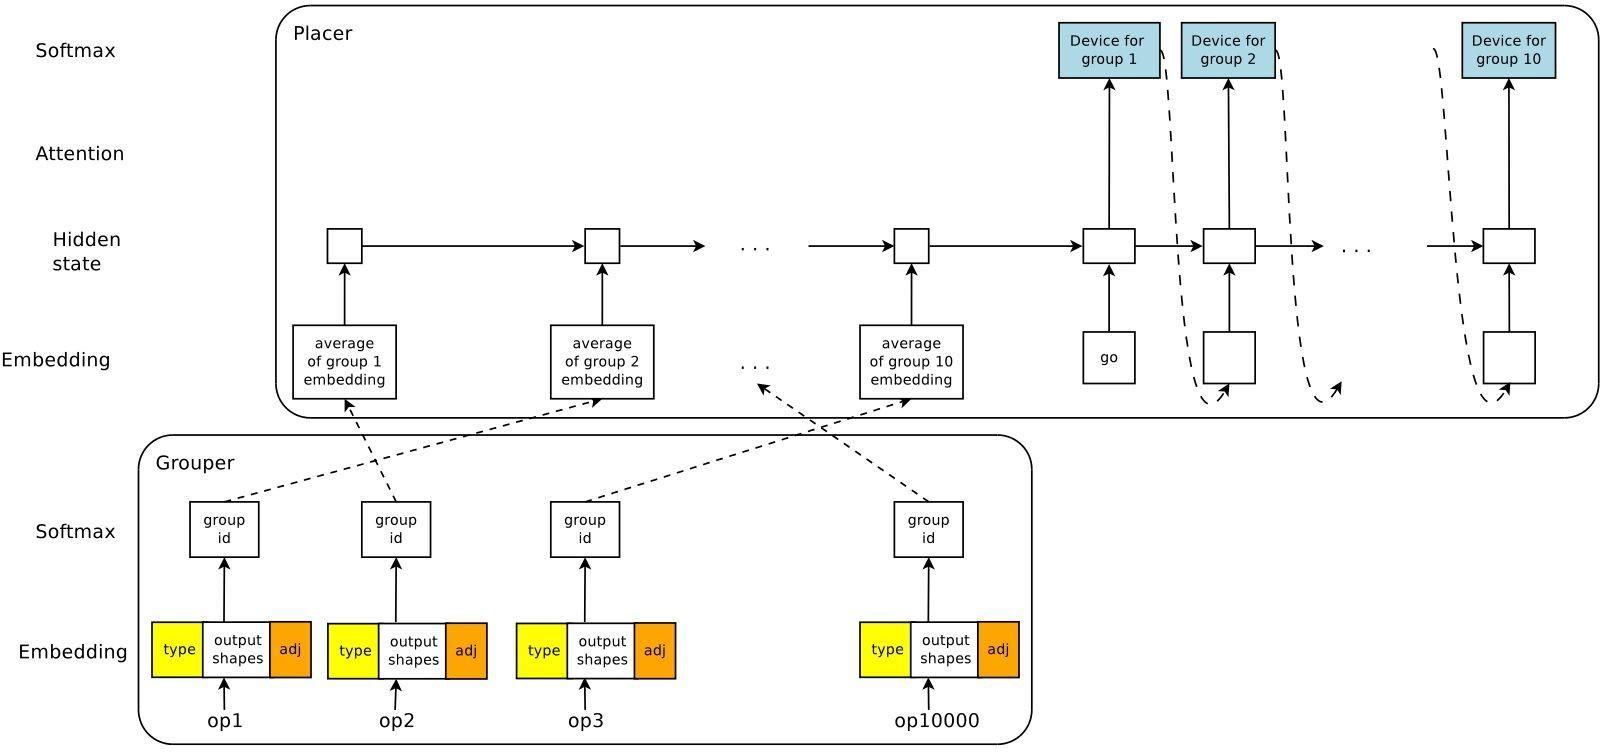
\includegraphics[width=\linewidth,height=0.78\textheight,keepaspectratio]{images/rl-real-world/figures/hierarchical.jpg}
\vfill
\end{frame}

% ---------------------------------------------------------------- Slide 39
\begin{frame}{Learned placement on NMT}
\centering
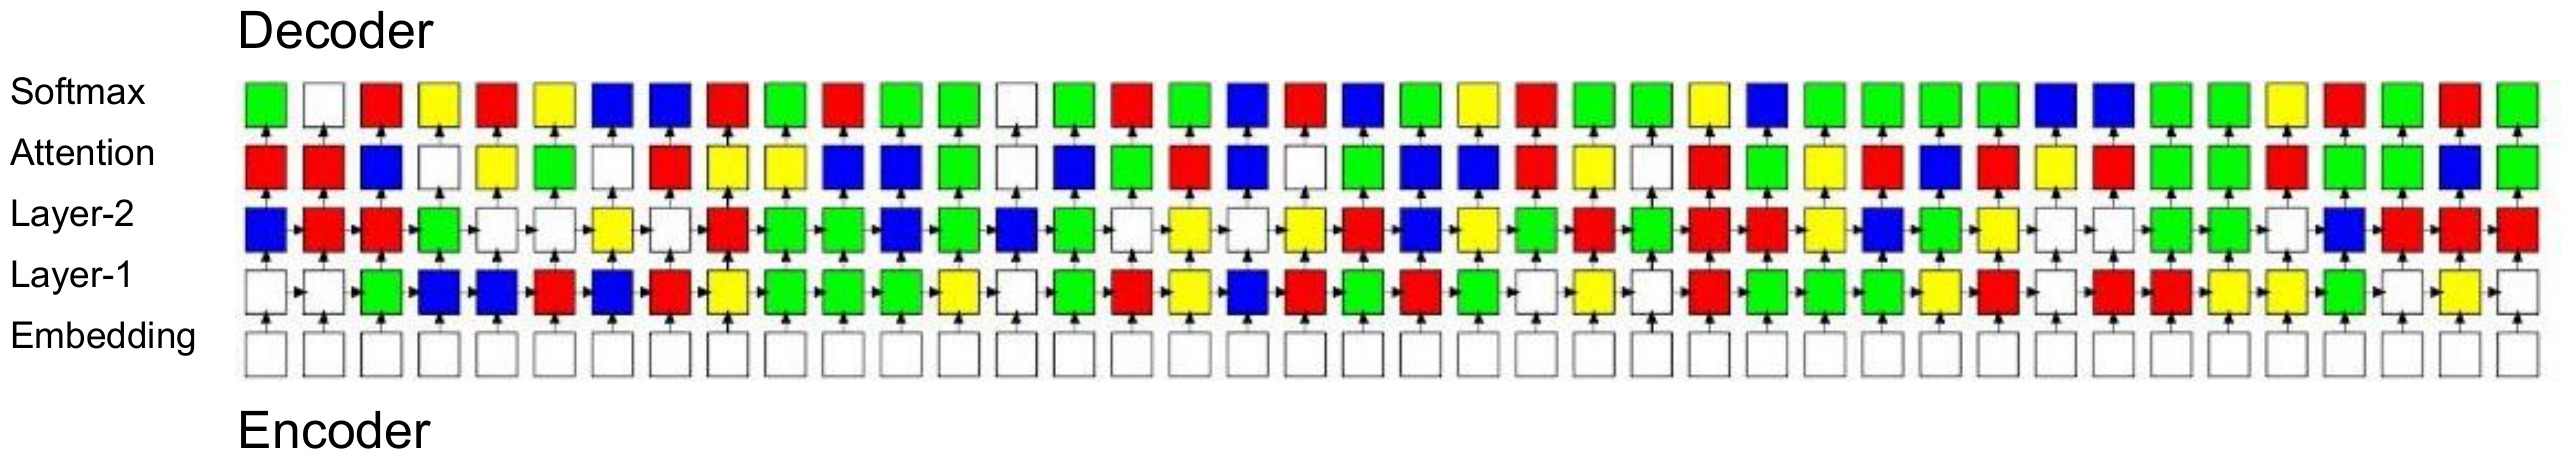
\includegraphics[width=0.96\linewidth,keepaspectratio]{images/rl-real-world/figures/nmt-decoder.jpg}\\[0.5em]
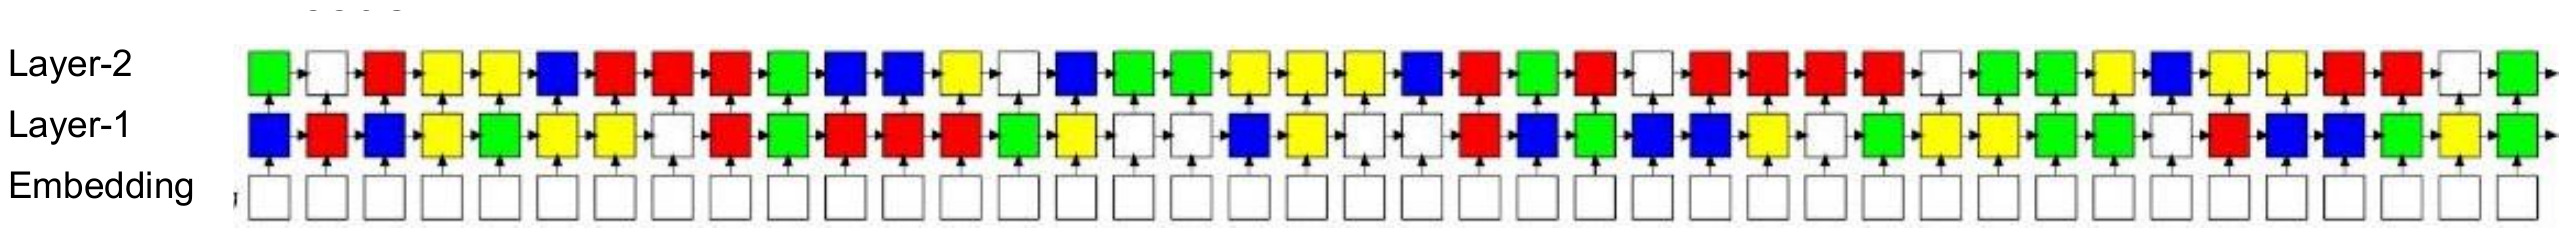
\includegraphics[width=0.96\linewidth,keepaspectratio]{images/rl-real-world/figures/nmt-encoder.jpg}
\vfill
{\scriptsize
White represents CPU (Ixion Haswell 2300).
Each other color represents a separate GPU (Nvidia Tesla K80).
Searching over a space of $5^{280}$ possible assignments.}
\footnote[0]{\scriptsize Mirhoseini et al. \href{https://arxiv.org/abs/1802.09756}{Hierarchical Planning for Device Placement}. ICLR 2018.}
\end{frame}

% ---------------------------------------------------------------- Slide 40
\begin{frame}{Profiling placement on NMT}
\vfill
\centering
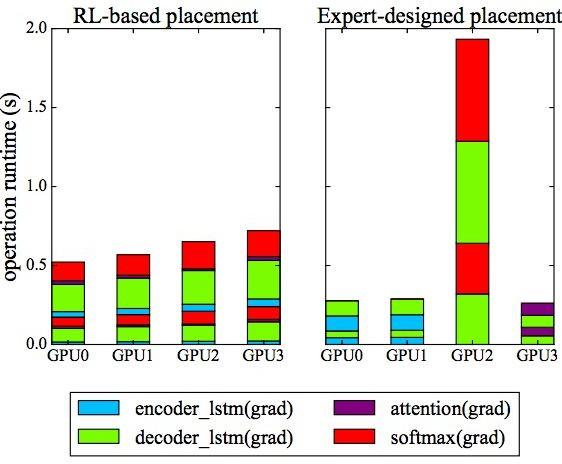
\includegraphics[width=\linewidth,height=0.78\textheight,keepaspectratio]{images/rl-real-world/figures/profiling.jpg}
\vfill
\end{frame}

% ---------------------------------------------------------------- Slide 41
\begin{frame}{Results (runtime in seconds)}
\vfill
\centering
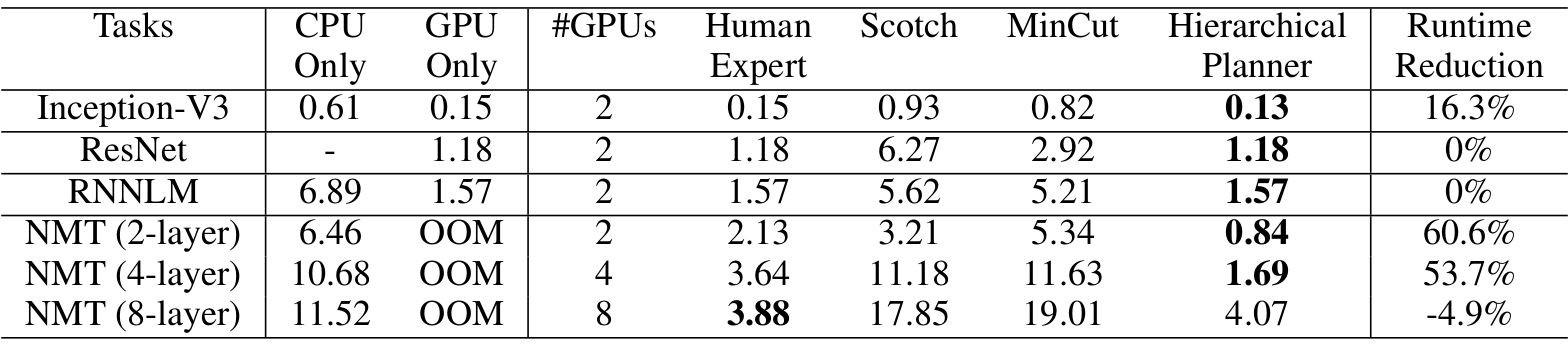
\includegraphics[width=\linewidth,keepaspectratio]{images/rl-real-world/figures/device-results.jpg}
\vfill
\end{frame}
